
%---------------------------------------------------------------------------
% Při prezentování nejvíc záleží na začátku. 
% Pro získání pozornosti na začátku veřejné řeči se doporučuje: říct nějakou statistiku; položit otázku (u státnic spíše řečnickou).

% HEROUT, Adam. Prezentování. Herout.net: Poznámky učitele, kouče, čtenáře. [online]. [cit. 2021-9-15]. Dostupné z: https://www.herout.net/blog/category/prezentovani/
%---------------------------------------------------------------------------

% - Uveďte posluchače do tématu své práce.
% - Řekněte něco málo o stavu před zahájením práce a jaké byly důvody pro její vypracování.
% - Nejlepší je vysvětlit motivaci pomocí schématu. Pokud musíte použít odrážky, tak super-stručné, abyste je nečetli, ale ony pouze tvořily kostru sdělení.

% Z této části prezentace musí posluchači dostat stručné a výstižné odpovědi na otázky:
%  A) Proč děláte, co děláte? K čemu je to dobré?
%  B) Co je cílem práce? Co má být výsledkem?

% Odolejte pokušení říkat banality a všeobecně známé informace.
% "Žijeme v době rozvoje mobilní výpočetní techniky, kdy každý má v kapse mobil" - je dokonale prázdné a hloupé sdělení, nic takového neříkejte, fakt to nikoho nezajímá.


% Nachazime se v dobe, kdy je vsechno na internetu, a to vcetne citlivych dat
% Vsechny vase soukrome zpravy, osobni udaje, vtipne fotky i mene vtipne fotky - vsechno to tam je
% A tenhle trend nezastavitelne roste, a tudiz roste i potreba, aby se tato data dostala jen do spravnych rukou
% Sdilene sluzby tedy musi vytycit presna pravidla pro pristup k datum, ktera ukladaji
% Mnozine takovych pravidel se rika policy/politika a pro uspesnou sluzbu je potreba ji mit pevne danou a zajistovat jeji dodrzovani
% Podle techto pravidel pak autorizovat jeji uzivatele k dany akcim
\begin{frame}
    \frametitle{Politiky přístupových práv}
    \begin{itemize}
        \item Citlivá data ve sdílených prostorech
        \item Autorizace
    \end{itemize}
\end{frame}

% Open Policy Agent je nastroj pro specifikaci a dodrzovani politiky
% Jeho hlavnim principem je decoupling, tedy oddeleni, politiky od softwaru sluzby, coz umoznuje mnohonasobne prehlednejsi a udrzitelnejsi spravu pristupovych prav
% Je vyuzivan napriklad Netflixem pro autorizaci internich API callu, dale v Cloudflare, nebo Pinterestu
% Pravidla politiky jsou specifikovana v deklarativnim jazyku Rego, ktery je navrzen se myslenkou maximalni uzivatelske privetivosti a jednoznacnosti
\begin{frame}
    \frametitle{Open Policy Agent (OPA)}
    \begin{columns}
        \column{0.3\textwidth}
        \begin{itemize}
            \item \emph{Decoupling} politiky a služby
            \item Policy as code
            \item Deklarativní jazyk \emph{Rego}
        \end{itemize}
        \column{0.7\textwidth}
        \input{img/opa-query-graph.tex}
    \end{columns}
    \vspace{1cm}
    % netflix - interni API cally
    % cloudflare - pro integraci Kubernetes/microservices
    Netflix, Cloudflare, Pinterest, ...
\end{frame}


%%%%%%%%                       02 - Cíle práce                      %%%%%%%%
%---------------------------------------------------------------------------
% Stručně uveďte cíle Vaší práce.
% Vhodné jsou max. 3 odrážky/věty s hlavními cíli.

% Někdy je motivace totožná s formulací cílů. Nenuťte se do dvou slajdů, když je správnější myšlenku vyjádřit jedním... 

% Formulujte, co je cílem:
%  - Jak se pozná úspěšný výsledek?
%  - Co jsou výstupy?
%  - Jaké vlastnosti má mít úspěšný výsledek?
%  - Kde to půjde použít?

% Lepší je bez použití odrážek:
%  - mít dostatečně dobrý obrázek, který budete svými slovy komentovat 
%  - na obrázku je vizuální sdělení, sdělení slovní dodáte pusou

% Je zbytečné říkat generická a obecná tvrzení: "Řešení by mělo být rychlé, spolehlivé a robustní" - toto jsou obecné požadavky na cokoli a informační hodnota sdělení je NULA - je to jen plýtvání časem a inteligencí.
% Mluvte konkrétně: Jaké konkrétní vlastnosti má mít Vaše řešení, co konkrétně znamená "robustní", co konkrétně znamená "spolehlivé"?

% Cilem moji diplomove prace je prevod jazyka Rego do SMT, coz umozni jeho naslednou analyzu
% Tento proces bude soucasti nastroje VeriRego, vyvijenem nasi fakultni vyzkumnou skupinou VeriFITem
\begin{frame}
    \frametitle{Cíle práce}
    Efektivní \emph{převod} Rego do \emph{SMT}

    \vspace{1cm}

    \centering
    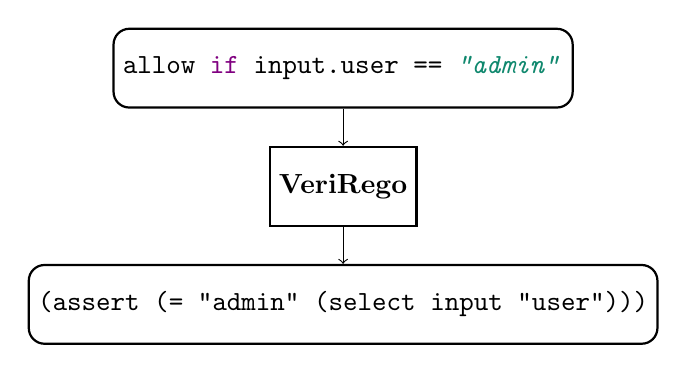
\begin{tikzpicture}[
        s/.style={draw,thick,rectangle,minimum height=10mm, minimum width=18mm},
        code/.style={draw,thick,rectangle,minimum height=10mm, minimum width=18mm,rounded corners=2mm},
    ]
    \tikzset{
        node distance=15mm,
    }
        \node[code] (in) { \texttt{allow \color{Purple}\textbf{if} \color{Black}input.user == \color{PineGreen}\textit{"admin"}} };
        \node[s,below of=in] (verirego) { \textbf{VeriRego}};
        \node[code,below of=verirego] (out) { \texttt{(assert (= "admin" (select input "user")))}};

        \draw[->]
            (in) edge (verirego)
            (verirego) edge (out);
    \end{tikzpicture}
\end{frame}

% Mozna se ptate, jestli podobne nastroje jiz existuji
% Nejvyznacnejsi jsou od Amazon Web Services, a to zaprve Cedar Analysis, kde Cedar je de facto omezenou odnosi Rego jazyka vyhradne navrzenou pro formalni verifikaci
% Dalsi ukazkou je Zelkova - analyzator IAM policies, ktery posuzuje, jestli je dana sluzba zcela verejna
% Existuji i dalsi priklady, kde vetsina funguje prave na prevodu do SMT, ale u tech nejrelevantnejsich se jedna o specifikacni jazyky, ktere maji omezenejsi schopnosti oproti Regu
% Pro samotne Rego jsem ve svem pruzkumu nenasel zadnou verejne znamou alternativu k nasemu nastroji
\begin{frame}
    \frametitle{Podobné nástroje}
    \begin{itemize}
        \item \emph{Cedar} Analysis (AWS Cedar politiky)
        \item \emph{Zelkova} (AWS IAM politiky)
    \end{itemize}

    \vspace{.5cm}
    
    \begin{itemize}
        \item Omezené specifikace pravidel
        \item SMT
    \end{itemize}
\end{frame}


%%%%%%%%                  03 - Informace o řešení                   %%%%%%%%
%---------------------------------------------------------------------------
% Cílem  obhajoby je podat zprávu o stavu projektu, nikoliv tedy držet přednášku na zadané téma. Mluvte o tom, co vy jste udělali, jaké jsou vaše výsledky. Mějte na slajdech formální pojmy, buďte přesní, definujte a odkazujte se.

% Prezentace nemusí a vlastně nemá obsahovat:
% -- Výklad použitých algoritmů apod. To patří do přednášky na dané téma, v prezentaci o stavu jen známé algoritmy uveďte podle jména, neznámé algoritmy třeba trochu přibližte, aby bylo zřejmo, o co jde, ale nevysvětlujte je podrobně. Není cílem, aby vaši posluchači algoritmu rozuměli a dokázali ho naprogramovat, ale aby měli představu, na čem pracujete a jak se vám to daří.
% -- Podrobnosti návrhu vašeho systému. Opět, posluchači nebudou váš systém hackovat, nepotřebují detailní strukturu tříd, názvy funkcí, jména souborů, datové formáty apod. Tyto věci uvádějte pouze v takové míře, která pomůže posluchačům udělat si představu, na čem pracujete a jak se vám to daří.

% HEROUT, Adam. Prezentování. Herout.net: Poznámky učitele, kouče, čtenáře. [online]. [cit. 2021-9-15]. Dostupné z: https://www.herout.net/blog/category/prezentovani/
%---------------------------------------------------------------------------

% - Uveďte, jaké zajímavé problémy jste v práci řešili.
% - Mělo by z toho být patrné, že je to závěrečná práce -- ne jen další projekt do předmětu -- tedy je v tom něco netriviálního, zajímavého a přínosného.
% - Raději dva nebo tři slajdy, které ukážete/vysvětlíte během 20 vteřin, než se snažit všechno "namastit" na jeden slajd.
% - Na slajdy je dobré dát vizuální informaci: vzorce, schemata, obrázky, diagramy. Slovní informaci můžete předat pusou. Je dokonale zbytečné a otravné mít na slajdu v odrážkách to samé, co se chystáte říct.
% - Titulek slajdu "Podstatné informace o řešení" je hodně generický. Ve skutečné Vaší prezentaci bude daleko lepší použít specifický titulek na každém ze slajdů, například: "Schéma neuronové sítě pro detekci frňáků", "Návrh nekonečného automatu", "Vytvořená datová sada" apod.

% Co jsou ale hlavni problemy pri prevodu Rega do SMT?
% Asi hlavni obtizi je expresivita jazyka, ktera umoznuje velke mnozstvi ruznych konstrukci, ktere, ac jsou snadno pochopitelne, mechanicky jsou narocne na zpracovani
% Roli hraje take dynamicke typovani jazyka, ktere muze byt v rozepri se staticky typovanym SMTLIBem, ktery podporuje vetsina solveru
% Co se tyce rozhodnutelnosti a efektivnosti pak hraji velkou roli kvantifikatory, ktere jsou v Rego jazyku valne pouzivane
\begin{frame}[fragile]
    \frametitle{Problematika}
    \begin{itemize}
      \item \emph{Expresivita} Rego jazyka
      \item \emph{Dynamické} typování
      \item Kvantifikátory
    \end{itemize}
    \vspace{.5cm}
\begin{lstlisting}[language=Rego]
package example

roles := graph.reachable(data.roles, input.user.role)

allow if {
  some role in roles
  data.priority[role] > 3
} else if {
  input.user.name == "admin"
}
\end{lstlisting}
\end{frame}

%%%%%%%%                    04 - Výsledky práce                     %%%%%%%%
%---------------------------------------------------------------------------
% Shrňte, jakých výsledků se Vám podařilo dosáhnout.
% Uveďte, jakým způsobem byla vyhodnocena funkčnost a správnost řešení.
% Buďte konkrétní: místo "Aplikace je otestovaná", řekněte, kým a jak byla testována, jaké byly výsledky testů.
% Místo "Úspěšnost detektoru je hodně dobrá" řekněte "Úspěšnost detektoru je 93 % mAP" nebo ještě radši ukažte tabulku se srovnáním oproti alternativním řešením.
% Pokud vyhodnocení sestávalo ze dvou nebo tří částí, může být vhodné rozdělit obsah na dva či tři slajdy. Při prezentování je ovšem potřeba se pohlídat, aby čas věnovaný každému slajdu byl adekvátně krátký a nedošlo k přetažení času.


% V soucasnem stavu je vyvijeny nastroj schopen typove inference, ktera umoznuje dalsi zpracovavani
% dale generovani odpovidajicich typu pro SMTLIB
% Co se tyce samotneho prevodu, uz je vyvinut na podporu ..., a schemat dokumentu, tedy jejich symbolicke reprezentaci
\begin{frame}
    \frametitle{Výsledky práce}
    \begin{itemize}
        \item Převod fragmentu jazyka Rego do SMT
        \item \emph{Návrh} a \emph{implementace} dvou analýz:
          \begin{itemize}
              \item Chyby za běhu
              \item Mrtvý kód
          \end{itemize}
    \end{itemize}
\end{frame}

% Jeste nas ceka prevod parametrickych pravidel a overeni rozhodnutelnosti fragmentu rego jazyka pro ruzne analyzi, coz bude doprovazeno i znacnym testovanim
\begin{frame}[fragile]
    \frametitle{Analýza - Chyby za běhu}
    Zápis rozdílných hodnot do stejné proměnné

    \vspace{.5cm}
    \begin{lstlisting}[language=Rego]
...

allow := true if {
  user.balance > input.cost
}

allow := false if {
  user.name in banned_users
}
\end{lstlisting}
    \vspace{.5cm}

  \textit{Analýza vrací konkrétní příklad vstupu}
\end{frame}

\begin{frame}[fragile]
    \frametitle{Analýza - Mrtvý kód}
    Podmínky, které nikdy neovlivní hodnotu proměnné

    \vspace{.5cm}
    \begin{lstlisting}[language=Rego, escapechar=|]
...

x if {
  y > 2
} else if {
  y < 4
} else if {
  |\textbf{\color{red}y == 3}|
}
\end{lstlisting}
  \hspace{5mm}
  \small\textit{Podmínka \textbf{if \{ y == 3 \}} je redundantní.}
    \vspace{.5cm}
\end{frame}

\begin{frame}
    \frametitle{Vyhodnocení}
    \begin{itemize}
        \item Experimentalní vyhodnocení na ručně sestavených příkladech
        \item Kombinace:
          \begin{itemize}
              \item Aritmetických funkcí
              \item Základních řetězcových operací
              \item Strukturovaných objektů
              \item Polí
          \end{itemize}
    \end{itemize}
\end{frame}

%%%%%%%%                      05 - Poděkování                       %%%%%%%%
%---------------------------------------------------------------------------
% Na tomto slajdu by měl být buď jeden velký, nebo více menších vhodně poskládaných obrázků.
% Vyberte to nejlepší, čím se chcete pochlubit - komise se na tento slajd bude dívat nejdéle ze všech slajdů.
% U tohoto slajdu ústně poděkujete za pozornost (ne nutně textem přes celý slajd) a komise pak bude mít prostor pro jeho prohlížení při čtení posudků.
%---------------------------------------------------------------------------

% Co padne na konci prezentace, je to, co posluchači budou brát v úvahu při následném rozhodování.

% HEROUT, Adam. Prezentování. Herout.net: Poznámky učitele, kouče, čtenáře. [online]. [cit. 2021-9-15]. Dostupné z: https://www.herout.net/blog/category/prezentovani/
%---------------------------------------------------------------------------

% Mockrat vam dekuji za udeleny cas a vasi pozornost, a prenechavam prostor pro diskuzi
\begin{frame}[fragile]
    \frametitle{Děkuji za pozornost!}
    \centering
    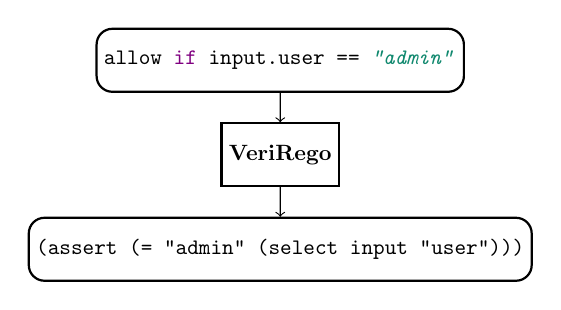
\begin{tikzpicture}[
        s/.style={draw,thick,rectangle,minimum height=10mm, minimum width=18mm},
        code/.style={draw,thick,rectangle,minimum height=10mm, minimum width=18mm,rounded corners=2mm},
        transform shape, scale=0.8
    ]
    \tikzset{
        node distance=15mm,
    }
        \node[code] (in) { \texttt{allow \color{Purple}\textbf{if} \color{Black}input.user == \color{PineGreen}\textit{"admin"}} };
        \node[s,below of=in] (verirego) { \textbf{VeriRego}};
        \node[code,below of=verirego] (out) { \texttt{(assert (= "admin" (select input "user")))}};

        \draw[->]
            (in) edge (verirego)
            (verirego) edge (out);
    \end{tikzpicture}

        \vspace{.5cm}

    \begin{lstlisting}[language=Rego, escapechar=|, basicstyle=\ttfamily\small]
...

x if {
  y > 2
} else if {
  y < 4
} else if {
  |\textbf{\color{red}y == 3}|
}
\end{lstlisting}
\end{frame}


%%%%%%%%                        06 - Otázky                         %%%%%%%%
%---------------------------------------------------------------------------
% U státnic student:
%   1) Prezentuje o své práci, skončí "Děkuji za pozornost!"
%   2) Předseda komise organizuje, co bude dál: čte se výtah z posudků.
%   3) Student zodpoví otázky, které oponent napsal do svého posudku.
%   4) Student odpovídá na otázky, které padnou v místnosti: od členů komise, ale třeba i od hostů.

% Pro bod 3) výše je vhodné mít připravené slajdy, které v odpovídání pomůžou:
%   A) Ukážou doslovný text otázky oponenta, student ji přečte, aby ji všichni znali, a pak na ni odpoví.
%   B) Budou obsahovat vizuální pomůcky k odpovědi.
%       a) Některé odpovědi na otázky žádnou vizuální pomůcku nepotřebují: student prostě řekne odpověď a všechno je jasné.
%       b) U jiných odpovědí je rozumné mít připravený obrázek, tabulku, graf, cosi, na čem odpověď jasně ukáže.

% Otázky oponenta nebývají myšlené jako "témata na přednášku". Pokud je možné odpovědět jednou větou, je to lepší, než mlžit okolo.
% Vizuální pomůcky často pomáhají ke stručné odpovědi: "Na schématu je vidět, že problém X řeším takto." A hotovo...

% Pokud k otázkám nebude potřeba žádná vizuální informace, je vhodné mít jednotlivé otázky jako odrážky na jediném slajdu.
% Pokud je otázek více a jsou k nim obrázky či grafy, je vhodné mít pro každou otázku jeden slajd - nahoře znění otázky, pod ním vizuální materiál.

\appendix{}
\begin{frame}
  \frametitle{Otázky oponenta}
  \begin{enumerate}
    \item Můžete uvést, která část architektury či funkcionality nástroje VeriRego je Vaším dílem?
      \item Jak to je s rozhodnutelností analýz pro Rego? Jsou rozhodnutelné nebo ne (a proč)? Pokud ne, máte fragment jazyka Rego, kde rozhodnutelnost lze garantovat?
  \end{enumerate}
  \bigskip
\end{frame}

\begin{frame}
  \frametitle{Otázky oponenta}
   \textit{  1. Můžete uvést, která část architektury či funkcionality nástroje VeriRego je Vaším dílem?}
  \bigskip

  \underline{Obě analýzy}, převod pravidel do SMT
  \bigskip
  \bigskip

  \small Dále jsem se podílel na: návrhu datových typů, podpoře pro nedefinované hodnoty, typové inferenci, reprezentaci uživatelských funkcí, přístupu do strukturovaných datových typů, ...
\end{frame}

\begin{frame}
  \frametitle{Otázky oponenta}
  \textit{2. Jak to je s rozhodnutelností analýz pro Rego? Jsou rozhodnutelné nebo ne (a proč)? Pokud ne, máte fragment jazyka Rego, kde rozhodnutelnost lze garantovat?}
  \bigskip

  Rego je navrženo, aby bylo rozhodnutelné:
  \begin{itemize}
    \item Zákaz rekurze
    \item Konečné vstupy
  \end{itemize}
  To ale neimplikuje obecnou rozhodnutelnost.
\end{frame}

\begin{frame}
  \frametitle{Otázky oponenta}
  \textit{2. Jak to je s rozhodnutelností analýz pro Rego? Jsou rozhodnutelné nebo ne (a proč)? Pokud ne, máte fragment jazyka Rego, kde rozhodnutelnost lze garantovat?}
  \bigskip

  Fragment, na kterém byly analýzy vystavěny, je rozhodnutelný:
  \begin{itemize}
    \item Aritmetické funkce
    \item Základní řetězcové operace
    \item Strukturované objekty
    \item Pole
  \end{itemize}
  \bigskip

  \small\textit{Očekáváme, že se podporovaný fragment může lišit pro různé analýzy.}
\end{frame}

%% Priklady 

\begin{frame}[fragile]
  \frametitle{Příklady: Kolize}
  \begin{lstlisting}[language=Rego, basicstyle=\ttfamily\small]
package e01

x := 1
x := 2
  \end{lstlisting}
  \textit{collision on values \textbf{1} and \textbf{2}} \\
  \texttt{input = \{ "count": 3, "word": "a" \}}

  \noindent\rule{\linewidth}{0.4pt}
  \begin{lstlisting}[language=Rego, basicstyle=\ttfamily\small]
package e02

x := 1 if input.count >= 1
x := 2 if input.count <= 1
  \end{lstlisting}
  \textit{collision on values \textbf{1} and \textbf{2}} \\
  \texttt{input = \{ "count": 1, "word": "a" \}}
\end{frame}

\begin{frame}[fragile]
  \frametitle{Příklady: Kolize}
\begin{lstlisting}[language=Rego, basicstyle=\ttfamily\small]
package e03

x := true if input.word == "Hello, World!"
x := false if contains(input.word, "!")
\end{lstlisting}
\textit{collision on values \true and \false} \\
\texttt{input = \{ "count": 2, "word": "Hello, World!" \}}
\end{frame}

\begin{frame}[fragile]
  \frametitle{Příklady: Kolize}
\begin{lstlisting}[language=Rego, basicstyle=\ttfamily\small]
package e04

y := 1
x := z if z := y-1
x := y if input.count > 1
\end{lstlisting}
\textit{collision on values \textbf{z} and \textbf{y}} \\
\texttt{input = \{ "count": 2, "word": "c" \}}
\noindent\rule{\linewidth}{0.4pt}

\begin{lstlisting}[language=Rego]
package e06

x := 1 if input.count == 1
x := 2 if input.count == 2
x := input.count
\end{lstlisting}
\textit{no collisions}
\end{frame}

% Subsume

\begin{frame}[fragile]
  \frametitle{Příklady: Mrtvý kód}
\begin{lstlisting}[language=Rego, escapechar=|]
package e01

x if input.count > 1
|\textbf{\color{red}x if input.count > 10}|
\end{lstlisting}

\noindent\rule{\linewidth}{0.4pt}
\begin{lstlisting}[language=Rego, escapechar=|]
package e02

x if {
  input.count > 1
} else if {
  |\textbf{\color{red}input.count > 10}|
}
\end{lstlisting}
\end{frame}

\begin{frame}[fragile]
  \frametitle{Příklady: Mrtvý kód}
\begin{lstlisting}[language=Rego, escapechar=|]
package e03

x if contains(input.word, "X")
|\textbf{\color{red}x if contains(input.word, "XX")}|
\end{lstlisting}

\noindent\rule{\linewidth}{0.4pt}
\begin{lstlisting}[language=Rego, escapechar=|]
package e05

arr := [0,0,1,1,0,1]
x if arr[input.count] == 1
|\textbf{\color{red}x if input.count == 3}|
x if input.count == 4
\end{lstlisting}
\end{frame}

% Jaka je mnozina povolenych dokumentu danou politikou?
% Jelikoz se interpretace bude nachazet v SMT, muzeme vstup specifikovat symbolicky, napriklad, ze ocekavame polozku user jako String.
% Zpracovani VeriRegem a nasledne SMT solverem nam pote nevrati jednu odpoved, ale model vsech moznych odpovedi
% Zaroven, jestli je symbolicky vstup v dane politice neprijatelny, muzeme z SMT solveru ziskat patricny protipriklad
\begin{frame}
  \frametitle{Analýza - Symbolická exekuce (návrh)}
    \begin{center}
        \textit{"Jaká je množina povolených dokumentů?"}
    \end{center}
    \vspace{.5cm}
    \centering
    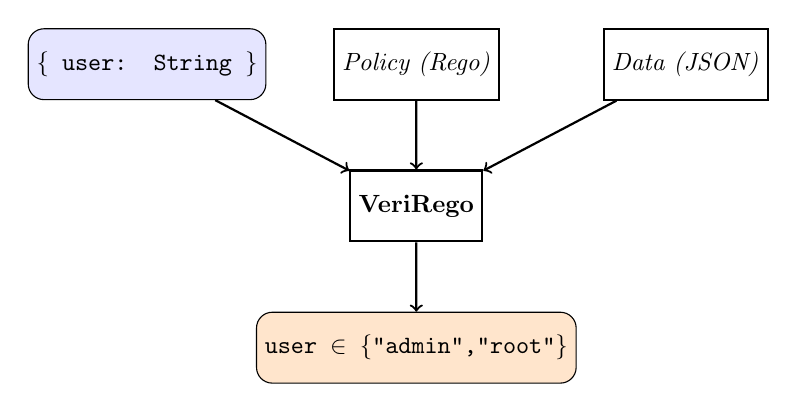
\begin{tikzpicture}[
            s/.style={draw,thick,rectangle,minimum height=10mm, minimum width=18mm},
            code/.style={draw,fill=blue!10,rectangle,minimum height=10mm, minimum width=18mm,rounded corners=2mm},
            e/.style={fill=gray!50},
            xsh/.style={xshift=15mm},
            transform shape, scale=0.9
        ]

        \tikzset{
            node distance=20mm,
        }

        \node[code] (input) {\texttt{\{ user: \textbf{String} \}}};
        \node[s,right of=input,xshift=18mm] (policy) {\textit{Policy (Rego)}};
        \node[s,right of=policy,xshift=18mm] (data) {\textit{Data (JSON)}};
        \node[s,below of=policy] (OPA) {\textbf{VeriRego}};
        \node[code,fill=orange!20,below of=OPA] (output) {\texttt{user $\in$ \{"admin","root"\} }};
        % \node[s,below of=OPA] (output) {\textit{Output decision \textbf{(model)}}};

        \draw[->,thick]
        (input) edge (OPA)
        (policy) edge (OPA)
        (data) edge (OPA)
        (OPA) edge (output)
        ;

    \end{tikzpicture}

    \vspace{.5cm}
    + vracení protipříkladů
\end{frame}

% Dalsim vyuzitim je pote porovnani politik mezi sebou
% Muzeme se naprikklad ptat, zdali je novejsi politika striktnejsi, nez predchozi
% Toho by se dalo v SMT dosahnout ziskanim formuli popisujicich obe politiky a otazkou, jestli pro vsechny mozne instance vstupu platnost v jedne politice implikuje platnost v druhe politice
\begin{frame}
    \frametitle{Analýza - Porovnání politik (návrh)}
    \begin{center}
        \textit{"Je jedna politika striktnější než druhá?"}
    \end{center}
    \vspace{.5cm}
    \centering
    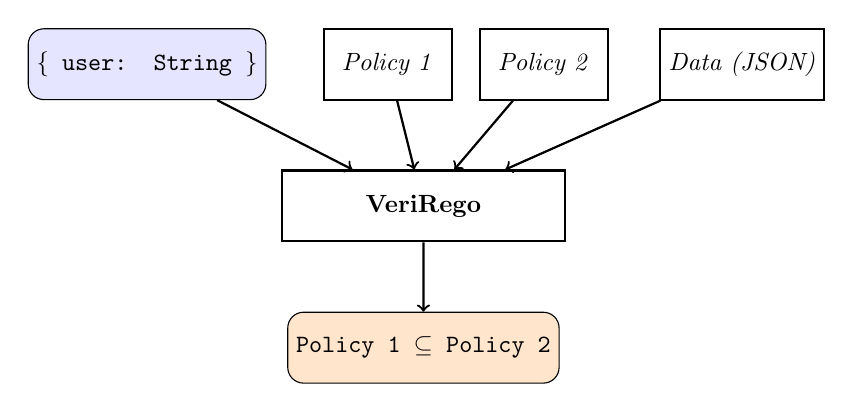
\begin{tikzpicture}[
            s/.style={draw,thick,rectangle,minimum height=10mm, minimum width=18mm},
            code/.style={draw,fill=blue!10,rectangle,minimum height=10mm, minimum width=18mm,rounded corners=2mm},
            e/.style={fill=gray!50},
            xsh/.style={xshift=15mm},
            transform shape, scale=0.9
        ]

        \tikzset{
            node distance=20mm,
        }

        \node[code] (input) {\texttt{\{ user: \textbf{String} \}}};
        \node[s,right of=input,xshift=14mm] (policy1) {\textit{Policy 1}};
        \node[s,right of=policy1,xshift=2mm] (policy) {\textit{Policy 2}};
        \node[s,right of=policy,xshift=8mm] (data) {\textit{Data (JSON)}};
        \node[s,below of=policy1,minimum width=40mm,xshift=5mm] (OPA) {\textbf{VeriRego}};
        \node[code,fill=orange!20,below of=OPA] (output) {\texttt{Policy 1 $\subseteq$ Policy 2}};

        \draw[->,thick]
        (input) edge (OPA)
        (policy1) edge (OPA)
        (policy) edge (OPA)
        (data) edge (OPA)
        (OPA) edge (output)
        ;

    \end{tikzpicture}
\end{frame}

